\documentclass[12pt]{article}

\usepackage[margin=1in]{geometry}
\usepackage{graphicx}
\usepackage{multirow}
\usepackage{subcaption}

\title{Low-Power Machine Learning}
\author{Joe Redmon and Calvin Loncaric}
\date{June 12, 2014}

\begin{document}

\maketitle

\section{Introduction}

Low-power computing devices are becoming increasingly relevant. As computing
becomes more common, it will be more and more important to reduce power costs.
Low-power devices can be deployed in more areas where a steady supply of
electricity may be harder to come by. Lowering power requirements can increase
usability by increasing battery life. Battery-free devices that harvest energy
from ambient sources (such as radio waves) can be manufactured more cheaply
than battery-powered devices. As they have no battery, they are also more
environmentally friendly and require significantly less maintenance.

Previous work has established that gesture recognition on low-power devices is
possible \cite{allsee}. This means that low-power devices can augment or
replace high-power gesture recognition technologies. However, the set of
gestures available must be hard-coded in advance and be carefully tuned for the
low-power environment. In this work we seek to remove this restriction by doing
simple machine learning on the device itself, enabling users to train new
gestures and removing the need for implementors to devise specialized
algorithms and heuristics.

Machine learning has been successfully applied in almost every real-world
setting: control systems, computer vision, speech recognition, language
processing, signal processing, information retrieval, and many other domains.
Given its ubiquity, bringing machine learning to low-power devices could have
other applications as well. Control systems---such as those in thermostats---%
can learn patterns in their environment to better predict temperature changes
and adjust in advance. In the context of localization, machine learning could
enable devices to learn to differentiate various different locations by using
various sensors (as in SurroundSense \cite{surroundsense}). By pressing a
button a user could effectively train a new relevant location into the device.

Our work focuses on gesture recognition and has resulted in a small working
prototype based on the MSP430 line of low-power CPUs. By pressing buttons the
user can train a gesture into the prototype by performing it only twice.

\section{Background and Related Work}

There is some previous work on machine-learning in low-power environments,
but not much, and none of it achieves our energy usage goals (under 50{$\mu$}W
of average usage).

Machine learning typically takes place in two phases. In the first phase
(``learning''), training data is used to construct a model. The model captures
with relatively little data the relationships in the training data and is used
in the second phase (``deployment'') along with input data to classify inputs
or predict outputs.

There has been previous work on producing models for low-power environments
\cite{low-power-models} but this work relies on a powerful external system to
produce the model in the first place. This makes it inappropriate for our
domain, as learning cannot be performed on the device itself.

Other groups have attempted to make learning low-power by producing dedicated
hardware \cite{ml-on-a-chip}. This work, while orders of magnitude more
power efficient than conventional hardware, still uses several
orders of magnitude more power than we would like. Their hardware requires
roughly 47300{$\mu$}W of power to run. Dedicated hardware could become
important, but we would prefer an approach that runs on general-purpose
hardware so the device can be used for other things when learning is not taking
place.

A simpler learning algorithm that is still relatively high-accurracy is
required.

\section{Implementation}

Our implementation uses a two-phase procedure to learn to recognize gestures. First it learns the ground truth for the gesture and then it estimates the size of the space that should be classified as the gesture. Subsequent gestures are compared to this space to see if they match the trained gesture. The whole training and recognition procedure takes place on low power hardware that is suitable for RF powered devices.

\subsection{Hardware}
For prototyping our algorithm we used a MSP430 microcontroller on a LaunchPad development board and a MMA8452 accelerometer. The MSP430 consumes 500{$\mu$}W of power during active operation, but only 0.1{$\mu$}W when it is in low power mode. The MMA8452 uses 16{$\mu$}W of power when collecting samples. Sampling and processing both happen in a one off manner and are driven by user input so the system is usually in low power mode.

These low-power components introduce some difficult constraints. In particular, common operations like multiplication and division are prohibitively expensive. Our approach is intentionally designed to avoid multiplication.

\subsection{Training}
When the user presses the input button, the device begins recording movement from the accelerometer. The first time the button is pressed, the sample is saved as the ground truth of the gesture. We sample for 2 seconds at 12.5 Hz, obtaining 25 readings. However, only the middle 15 (1.2 seconds) are used to eliminate noise at the beginning or end of the gesture.

The second time the button is pressed, the user performs the same action during the same time frame. We slide the ground truth gesture over the second buffer and find the window with the smallest difference:

\begin{equation}
\label{eq:norm}
\delta = \min_i \|V_{test}[i:i+15] - V_{truth} \|_1
\end{equation}

Using this $\delta$ we calculate our threshold $T = 1.5*\delta$

\subsection{Testing}
The full gesture model is specified by the ground truth vector $V_{test}$ and the threshold $T$. When the user presses the button again, we sample from the accelerometer and use equation \ref{eq:norm} to find the smallest overlap $\delta_{test}$. If $\delta_{test} < T$ than we classify the gesture as matching the trained gesture. If not, we reject it.

\begin{figure}[h]
\begin{center}
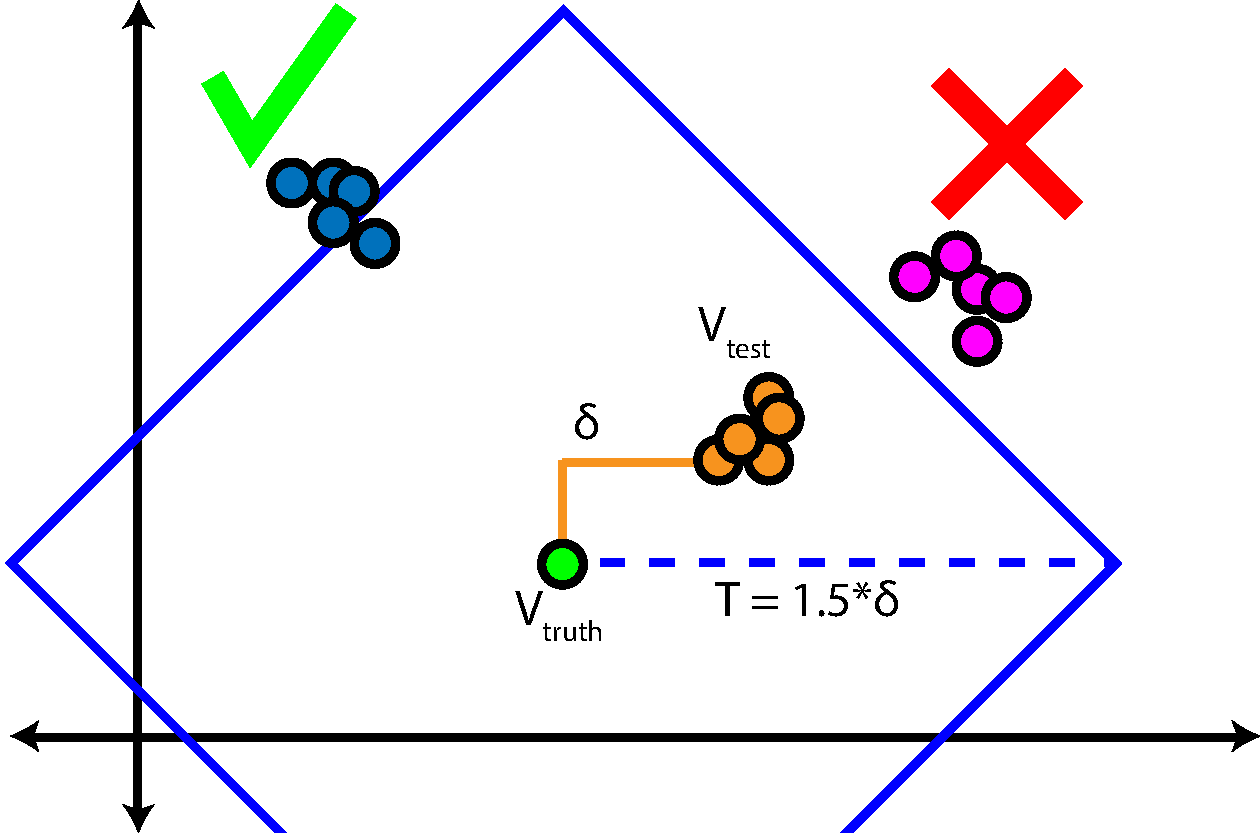
\includegraphics[width=.7\linewidth]{graph}
\end{center}
\caption{Our learning procedure. We learn the ground truth $V_{truth}$ and the threshold $T$. New examples are classified positive or negative based on their closest subvector.}
\label{graph}
\end{figure}


\begin{figure}[h!]
  \begin{center}
    \includegraphics[width=0.3\textwidth]{device-original.jpg}
  \caption{The prototype. Batteries are included on the back side.}
  \end{center}
\end{figure}

\section{Results and Discussion}

\begin{table}[h!]
\begin{center}
    \begin{tabular}{cc|cccc}
    & & \multicolumn{4}{c}{Trained} \\
    & & stab & swipe & loop & tilt \\
    \hline
    \multirow{4}{*}{Performed} & stab & 30 & 0 & 0 & 0  \\
    & swipe & 0 & 19 & 0 & 0 \\
    & loop & 0 & 0 & 30 & 0 \\
    & tilt & 0 & 0 & 0 & 21
    \end{tabular}
    \caption{Accuracy data. Columns indicate which gesture was
    trained into the device, and rows are which gesture was performed. Cells
    contain the number of positive recognitions for the ``performed'' gesture
    when trained on the ``trained'' gesture. Each
    cell was tested a total of 30 times. Each gesture was trained only once
    and then all rows were tested in order. Overall accuracy is 83\% with no
    false positives.}
    \label{tbl:data}
\end{center}
\end{table}

\begin{figure}[h!]
\begin{center}
    \begin{subfigure}[b]{0.2\textwidth}
            \includegraphics[width=\textwidth]{gesture-stab.png}
            \caption{Stab}
            \label{fig:stab}
    \end{subfigure}
    \begin{subfigure}[b]{0.2\textwidth}
            \includegraphics[width=\textwidth]{gesture-swipe.png}
            \caption{Swipe}
            \label{fig:swipe}
    \end{subfigure}
    \begin{subfigure}[b]{0.2\textwidth}
            \includegraphics[width=\textwidth]{gesture-loop.png}
            \caption{Loop}
            \label{fig:loop}
    \end{subfigure}
    \begin{subfigure}[b]{0.2\textwidth}
            \includegraphics[width=\textwidth]{gesture-tilt.png}
            \caption{Tilt}
            \label{fig:tilt}
    \end{subfigure}
    \caption{Gestures performed. ``Stab'' is a forward then a backward motion.
    ``Swipe'' is a left then a right motion. ``Loop'' is a counterclockwise
    circle. ``Tilt'' is a 45-degree turn around the forward axis, then a return
    to normal.}
    \label{fig:gestures}
\end{center}
\end{figure}

\begin{table}
\begin{center}
    \begin{tabular}{c|c}
    Task & Energy Usage \\
    \hline
    idle & 6.6$\mu$W \\
    collecting & 10980$\mu$W \\
    LED light & 13230$\mu$W \\
    \end{tabular}
    \caption{Energy usage information for our prototype at 3.3 volts. ``Idle''
    is when the prototype is doing nothing (not even collecting accelerometer
    data). ``Collecting'' is when the prototype is sampling data from the
    accelerometer. ``LED light'' is when the prototype is lighting up an LED to
    inform the user of a result.}
    \label{tbl:power}
\end{center}
\end{table}

Table \ref{tbl:data} shows collected accuracy data for our prototype for the
gestures listed in figure \ref{fig:gestures}. The data was collected by one of
the authors by training the device on a gesture and then performing each of
the other gestures thirty times. The table reports the number of positive
identifications.

The prototype had an overall 83\% accuracy with no false positives. These
results are not surprising: when training the device it is very easy to perform
exactly the same gesture twice in a row, so it learns a very strict threshold.
Subsequent gestures tend to deviate more significantly from the first few,
leading to a low overall recognition quality. Adjusting the threshold tolerance
could improve this at the risk of introducing false positives.

Another source of difficulty in recognition is strict orientation dependence.
Since multiplication is prohibitively expensive we cannot compute a dot product
of subsequent accelerometer data (to examine just the change in direction). Our
model requires that the gesture be performed in the exact same orientation
every time, so slight variations in direction can cause recognition failures.
(For instance, when performing the swipe gesture, the user must be careful not
to drift too far forward or backward while swiping.) Orientation dependence is
a blessing and a curse: it means that ``swipe'' is different from ``stab'' (and
in general we can differentiate more gestures) but it also makes it more
difficult to recognize a variation on the same gesture.

Our power usage information is shown in table \ref{tbl:power}. While these
numbers are \emph{significantly} higher than what we predicted based on our
hardware, we attribute them to poor circuit design and point out that our
components can certainly be used more effectively. Power usage can also be
improved by reducing various overheads: while collecting power usage data,
our prototype still lights up a small LED to indicate that work is taking place
and still writes data to the serial port for debugging.

\section{Conclusion and Acknowledgements}
We have shown that machine learning on low-power devices is certainly possible,
albeit limited. Our initial results are promising, with a somewhat high
recognition accuracy despite a very simple algorithm. Plenty of future work
remains to devise new algorithms and reduce power usage. We suggest two
directions for future researchers: looking at ways to reduce the amount of
data collected and ways to construct a more power-efficient prototype that
reflects what the hardware is capable of.

We would like to thank Bryce Kellogg for his invaluable assistance during this
project. He helped us get the hardware set up and measure power usage
information, and without his help we would not have gotten as far as we did.

\bibliography{bibliography}
\bibliographystyle{plain}

\end{document}
